\documentclass[11pt, a4paper]{article}
\usepackage[margin=1.1in]{geometry}	% edit margins
\usepackage{amsmath}			% for math symbols
\usepackage{graphicx}			% including figures
\usepackage{float}			% placing figures at specific location
\usepackage{amssymb}			% math symbols
\usepackage{color, soul}			% for highlighting
\usepackage{mathtools}			% for text over equals sign
\newcommand\ivtequal{\stackrel{\mathclap{\normalfont\scriptsize\mbox{FVT}}}{=}}
% \usepackage{./use/mcode}		% for including code


\begin{document}

\title{Final Project: Orbit Determination\\ ASEN 5044 Statistical Estimation}
\author{Keith Covington\\Connor Ott}
\date{December 18, 2019}
\maketitle



%%%%%%%%%%%%%%%%%%%%%%%%%%%%%%%%% INTRODUCTION  %%%%%%%%%%%%%%%%%%%%%%%%%%%%%%%%%
\section*{Introduction}
In order to keep track of Earth-orbiting objects, a typical observation scheme includes ground stations which measure range and range-rate to a passing satellite. 
These measurements, when combined with the known locations of the stations, allows for precises estimates of a satellites orbit state. 
In addition to an orbit estimate, it's usually useful to quantify the the uncertainty in the estimate. 
This quantity is a based on the uncertainty in the motion of the satellite in orbit, and the uncertainty in the incoming measurements. 
Neither of these uncertainties are necessarily known.
In order to accurately predict an estimate uncertainty, both of these uncertainties must be balanced with each other. 
This is frequently carried out with predictor-corrector estimation algorithm such as the Linearized Kalman Filter (LKF) or Extended Kalman Filter (EKF.)

In this report, we explore the performance of the LKF and EKF on nonlinear systems with dynamic uncertainty (process noise) and measurement uncertainty (measurement nose.) 
In developing these algorithms, we assume the process and measurement noise are unknown.
We then iterate on different process noise and measurement noise covariance matrices and evaluate the algorithms using \_\_\_\_ (NEES) and \_\_\_\_ (NIS) tests until suitable values for uncertainty are found. 

\section{Part I. Basic System Analysis}

\subsection{CT Model Jacobians}

$\tilde{A}$
$$\left[\begin{matrix}0 & 1 & 0 & 0\\\frac{3\mu x_{1}^{2}}{\left(x_{1}^{2} + x_{3}^{2}\right)^{2.5}} - \frac{\mu}{\left(x_{1}^{2} + x_{3}^{2}\right)^{1.5}} & 0 & \frac{3\mu x_{1} x_{3}}{\left(x_{1}^{2} + x_{3}^{2}\right)^{2.5}} & 0\\0 & 0 & 0 & 1\\\frac{3\mu x_{1} x_{3}}{\left(x_{1}^{2} + x_{3}^{2}\right)^{2.5}} & 0 & \frac{3\mu x_{3}^{2}}{\left(x_{1}^{2} + x_{3}^{2}\right)^{2.5}} - \frac{\mu}{\left(x_{1}^{2} + x_{3}^{2}\right)^{1.5}} & 0\end{matrix}\right]$$

$\tilde{B}$
$$\left[\begin{matrix}0.0 & 0.0\\1.0 & 0.0\\0.0 & 0.0\\0.0 & 1.0\end{matrix}\right]$$

$\tilde{\Gamma}$
$$\left[\begin{matrix}0.0 & 0.0\\1.0 & 0.0\\0.0 & 0.0\\0.0 & 1.0\end{matrix}\right]$$

$\tilde{H}$ - Hmmm
$$\left[\begin{matrix}\frac{x_{1} - x_s}{\left(\left(x_{1} - x_s\right)^{2} + \left(x_{3} - y_s\right)^{2}\right)^{0.5}} & 0 & \frac{x_{3} - y_s}{\left(\left(x_{1} - x_s\right)^{2} + \left(x_{3} - y_s\right)^{2}\right)^{0.5}} & 0\\\frac{\left(- x_{1} + x_s\right) \left(\left(x_{1} - x_s\right) \left(x_{2} - \dot{x}_s\right) + \left(x_{3} - y_s\right) \left(x_{4} - \dot{y}_s\right)\right)}{\left(\left(x_{1} - x_s\right)^{2} + \left(x_{3} - y_s\right)^{2}\right)^{1.5}} + \frac{x_{2} - \dot{x}_s}{\left(\left(x_{1} - x_s\right)^{2} + \left(x_{3} - y_s\right)^{2}\right)^{0.5}} & \frac{x_{1} - x_s}{\left(\left(x_{1} - x_s\right)^{2} + \left(x_{3} - y_s\right)^{2}\right)^{0.5}} & \frac{\left(- x_{3} + y_s\right) \left(\left(x_{1} - x_s\right) \left(x_{2} - \dot{x}_s\right) + \left(x_{3} - y_s\right) \left(x_{4} - \dot{y}_s\right)\right)}{\left(\left(x_{1} - x_s\right)^{2} + \left(x_{3} - y_s\right)^{2}\right)^{1.5}} + \frac{x_{4} - \dot{y}_s}{\left(\left(x_{1} - x_s\right)^{2} + \left(x_{3} - y_s\right)^{2}\right)^{0.5}} & \frac{x_{3} - y_s}{\left(\left(x_{1} - x_s\right)^{2} + \left(x_{3} - y_s\right)^{2}\right)^{0.5}}\\\frac{- x_{3} + y_s}{\left(x_{1} - x_s\right)^{2} + \left(x_{3} - y_s\right)^{2}} & 0 & \frac{x_{1} - x_s}{\left(x_{1} - x_s\right)^{2} + \left(x_{3} - y_s\right)^{2}} & 0\end{matrix}\right]$$ 	


\subsection{DT Linearized Model Matrices}

\subsection{Simulated Nonlinear vs. Linearized System}
Figure \ref{fig:nlvl_s} shows the difference between propagating a small initial perturbation using full nonlinear dynamics and the above DT state transition matrices. 
These were gathered by propagating two orbits, a nominal and initially perturbed orbit, with full nonlinear dynamics using an RK45 integration method.
The difference between these orbits is shown by the blue line in Figure \ref{fig:nlvl_s}. 
The initial perturbation (difference between the initial states of the nonlinear trajectories described above) was then propagated using the linearized DT jacobians evaluated on the nominal trajectory. 
The linear propagation of the perturbation is shown in red. 
The nonlinear and linear perturbations stay near each other for the first half of an orbit, but quickly grow apart.
This indicates that the linearized dynamics are only appropriate for short time spans while the perturbed orbit remains relatively close to the nominal orbit where the DT jacobians are evaluated. 

\begin{figure}[H]
	\centering
	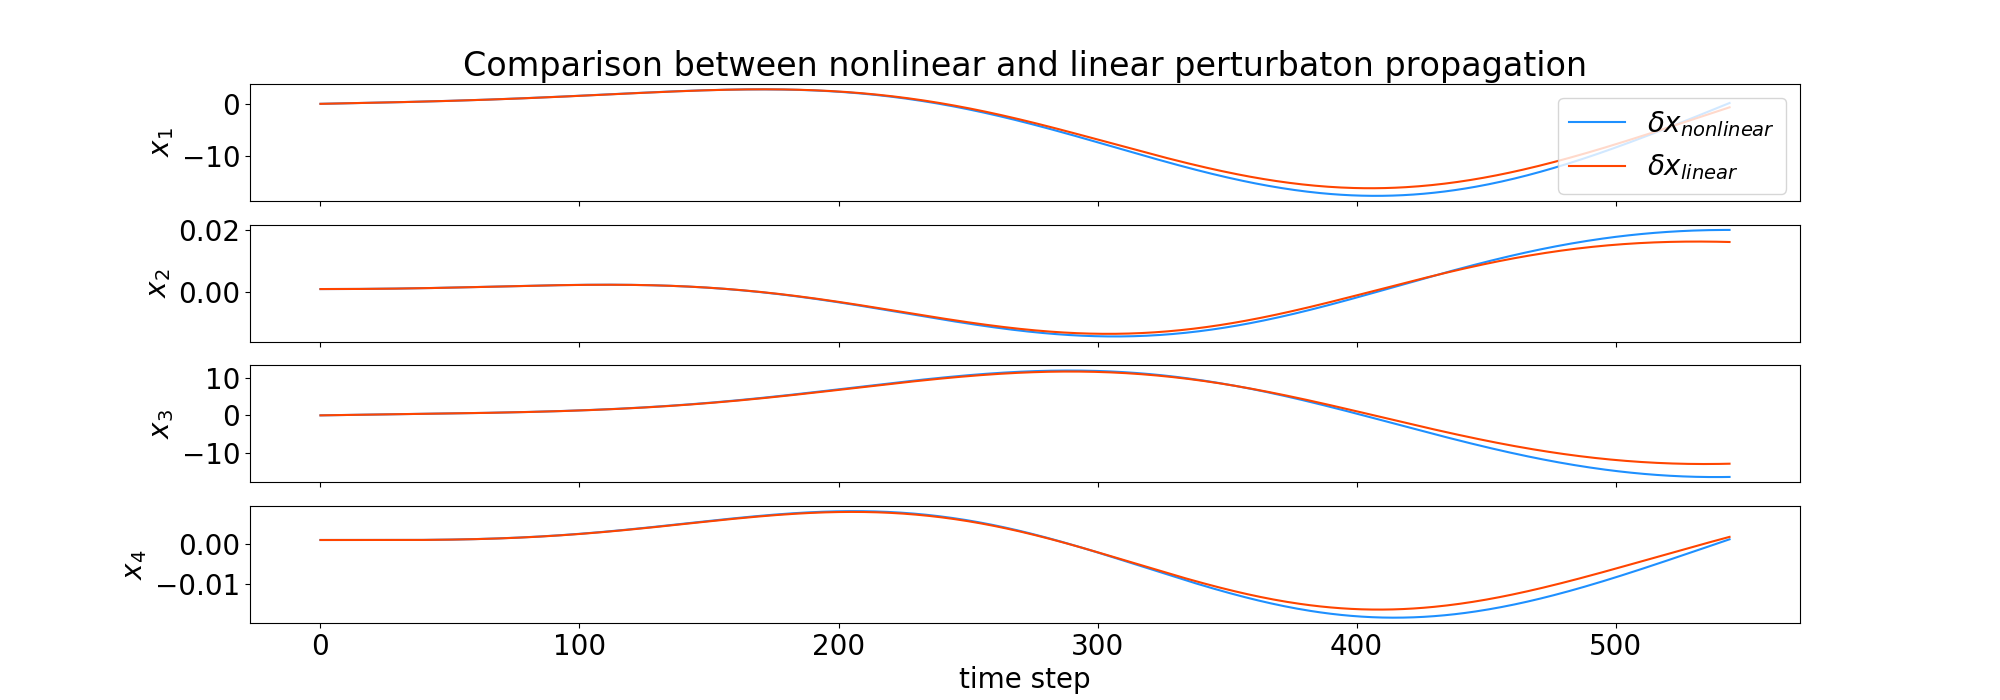
\includegraphics[width=0.8\textwidth]{./Figures/nonlvl_state.png}
	\caption{Comparision between nonlinear and linear perturbation propagation.}
	\label{fig:nlvl_s}
\end{figure}

We draw similar conclusions about the validity of the linearized measurement function from Figure \ref{fig:nlvl_m}.
As the perturbed orbit drifts further and further from the nominal orbit, the linearized dynamics and measurement function are unable to closely match the nonlinear dynamics. 

\begin{figure}[H]
	\centering
	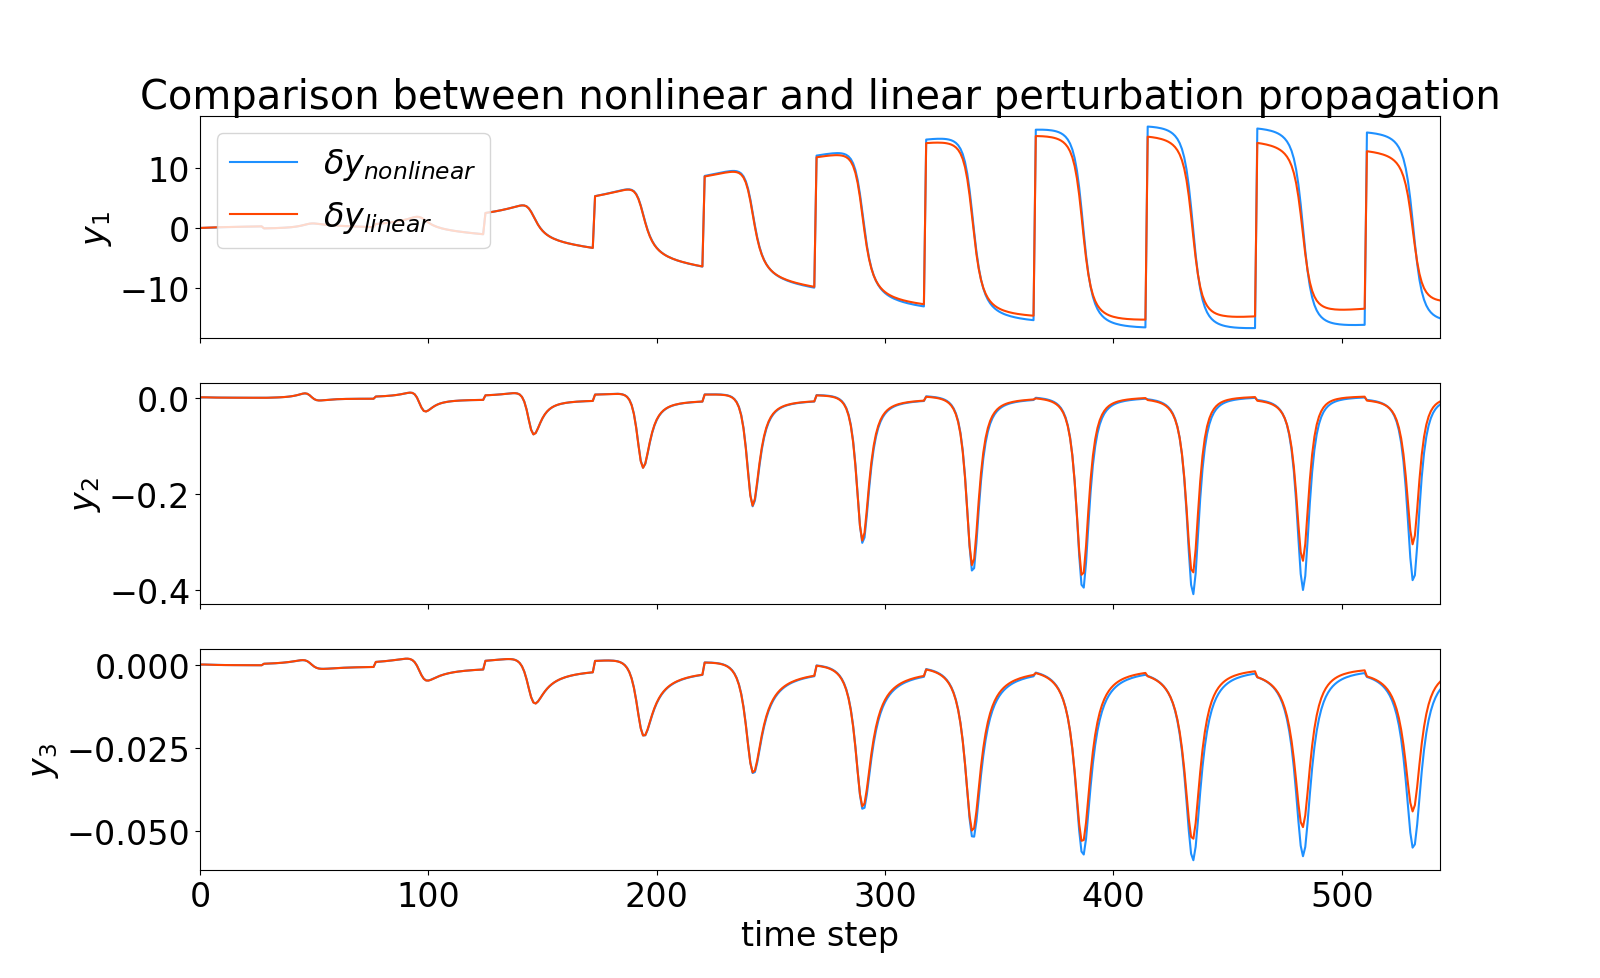
\includegraphics[width=0.8\textwidth]{./Figures/nonlvl_meas.png}
	\caption{Comparision between nonlinear and linear perturbation propagation.}
	\label{fig:nlvl_m}
\end{figure}


\section{Nonlinear Filtering}

\subsection{The Linearized Kalman Filter}
The LKF revolves around the concept of linearizing dynamics and measurement functions around a nominal trajectory at discrete time steps in the filter. 
This has its benefits in terms of simplicity and computational load, but suffers in terms of accuracy with relatively large deviations from the nominal trajectory. 
Figures \ref{fig:noisey_states} and \ref{fig:noisey_meas} show a typical noisey truth trajectory and accompanying noisey measurements as compared to the nominal, noiseless trajectory and measurements.  
Figure \ref{fig:lkf_est_zoom} shows the LKF estimate error and uncertainty bounds for the first 100 time steps (1e4 seconds) of the simulation. 
The filter performs adequately for these first 100 time steps.
However, as time goes on, and the truth trajectory deviates further from the nominal, the LKF is unable to estimate an accurate trajectory. 
Figure \ref{fig:lkf_est} shows the rapidly deriorating estimate error in the LKF.  
\begin{figure}[H]
	\centering
	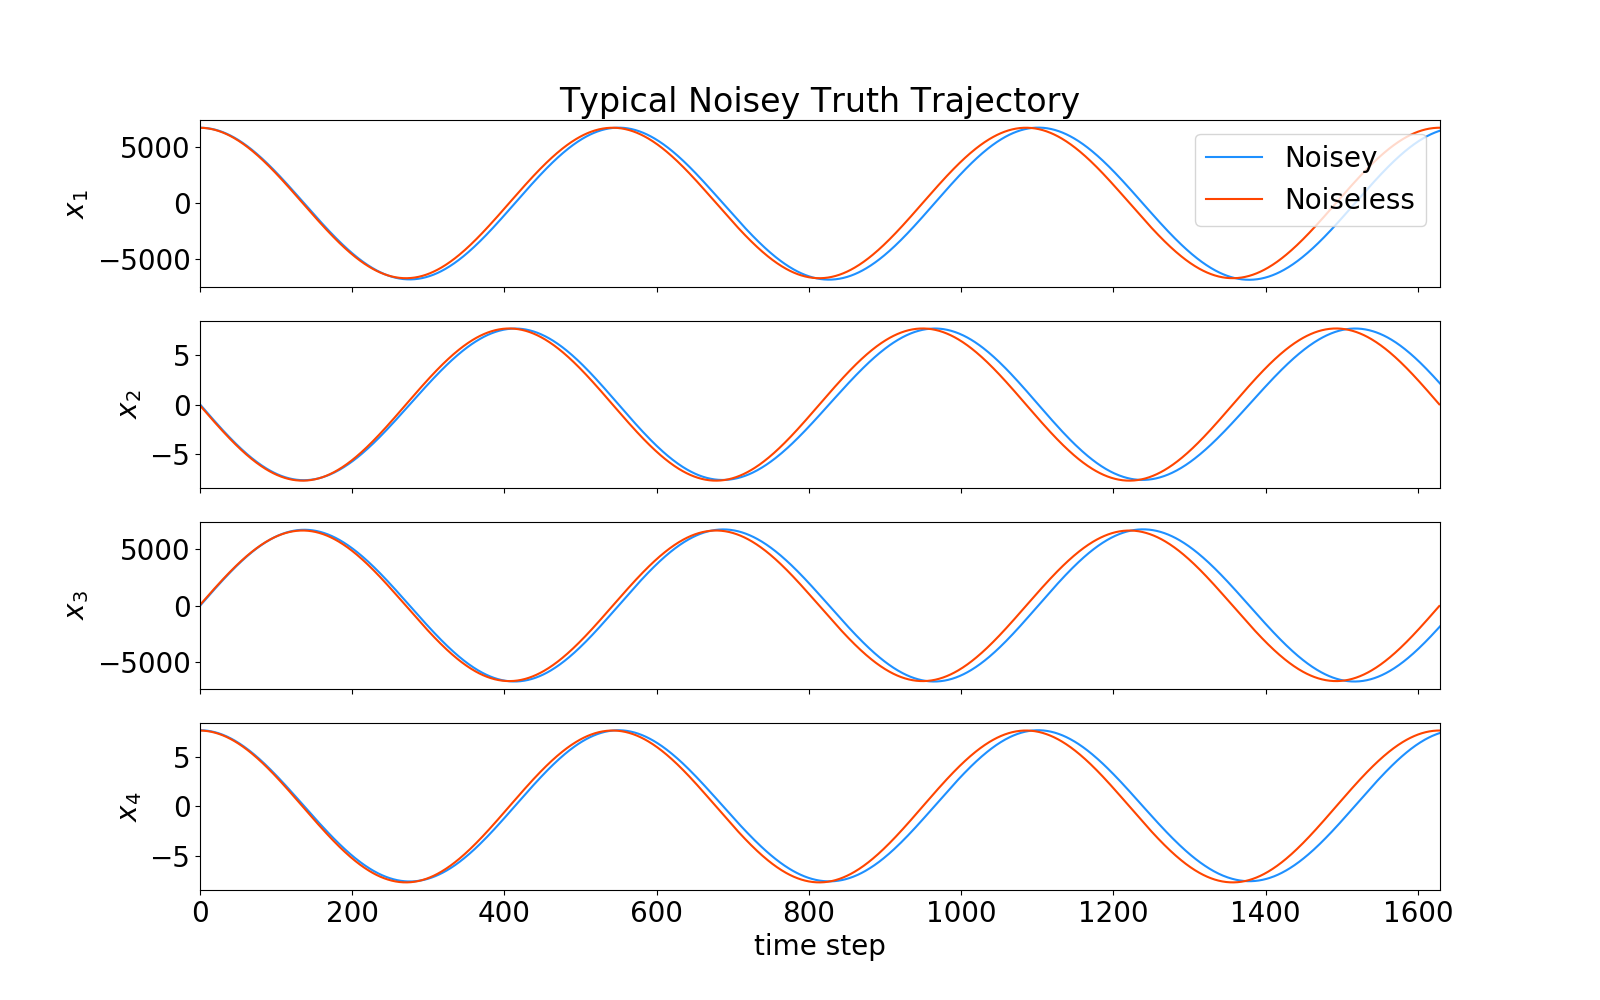
\includegraphics[width=\textwidth]{Figures/noisey_truth.png}
	\caption{Typical noisey trajecotory as compared to the nominal, noiseless trajectory.}
	\label{fig:noisey_states}
\end{figure}

\begin{figure}[H]
	\centering
	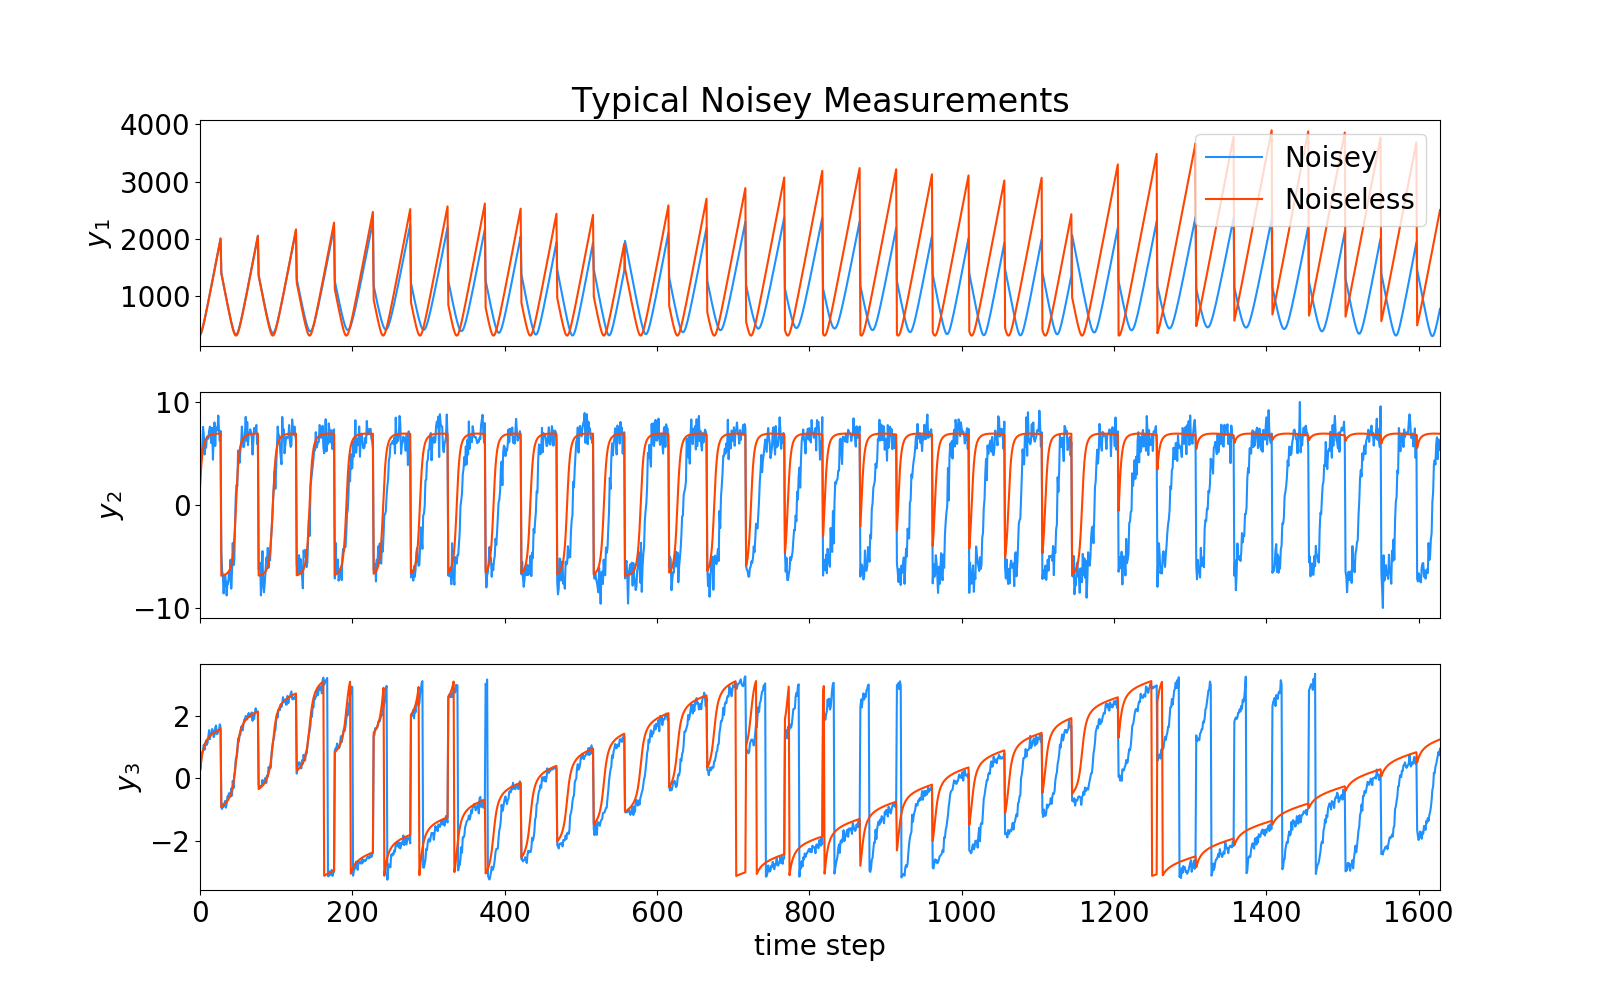
\includegraphics[width=\textwidth]{Figures/noisey_meas.png}
	\caption{Typical noisey measurements as compared to the nominal, noiseless measurements.}
	\label{fig:noisey_meas}
\end{figure}

\begin{figure}[H]
	\centering
	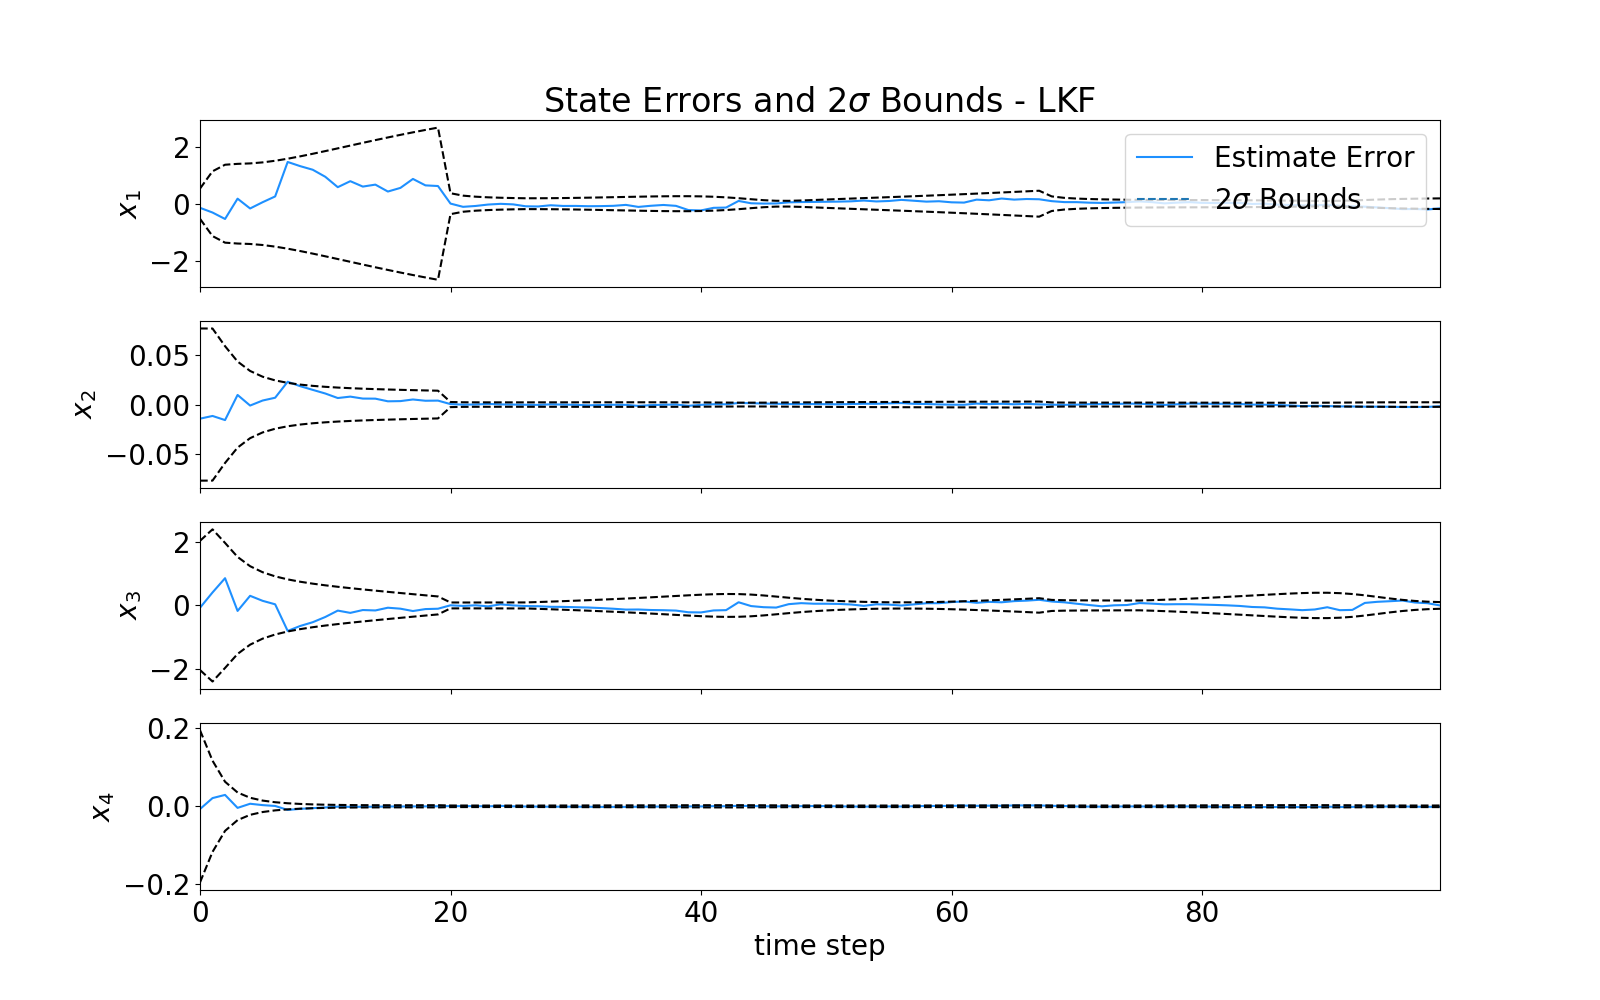
\includegraphics[width=\textwidth]{Figures/lkf_estimate_th_ZOOM.png}
	\caption{Typical LKF estimate for first 100 time steps (1e4 seconds or $\approx$1/5 of an orbit.)}
	\label{fig:lkf_est_zoom}
\end{figure}

\begin{figure}[H]
	\centering
	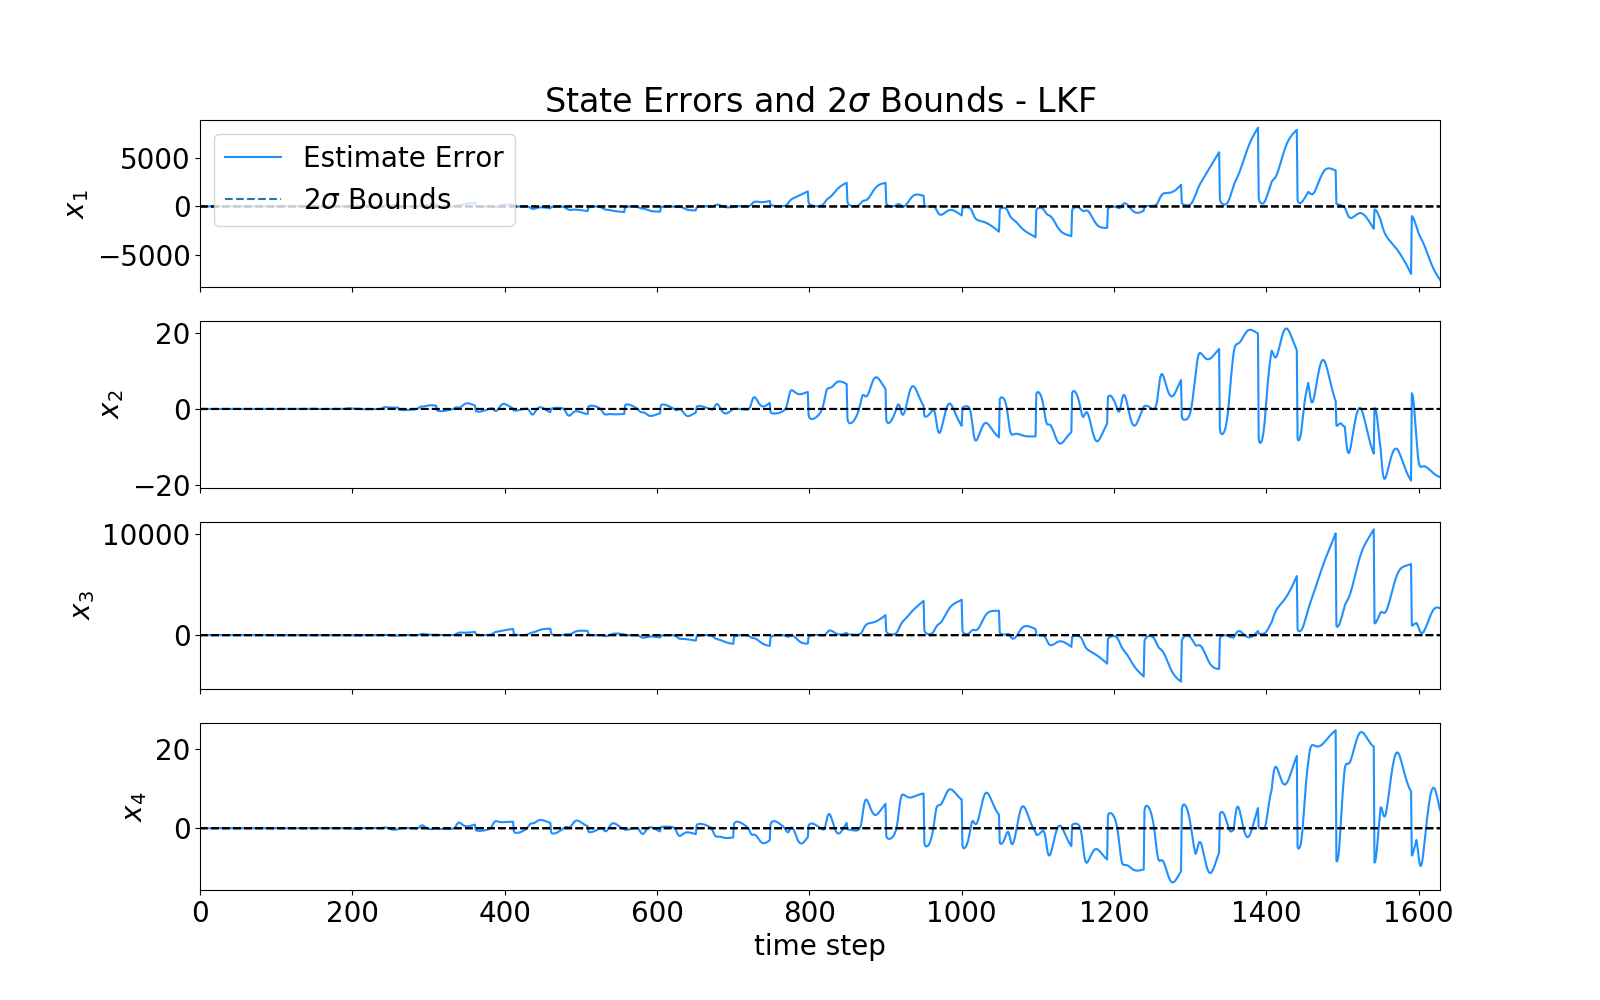
\includegraphics[width=\textwidth]{Figures/lkf_estimate_th.png}
	\caption{Typical LKF estimate for entire simulation.}
	\label{fig:lkf_est}
\end{figure}

\subsubsection{NEES and NIS Tests}
The following are results of NEES and NIS chi-square tests for an implementation of the LKF. 
\hl{list specs of the sim here when the final figures go in.} 
In the following figures, we plot NEES and NIS values from the filter at time k, averaged over N simulated trajectories. 
At each time step, the NEES and NIS values are expected to fall into 4 (NEES) or 3 (NIS) degree of freedom $\mathcal{X}^2$ distributions. 
As such, we expect values to fall within some range of the expecation of these distributions. 
For this study, we've chosen 95\% confidence bounds, which are denoted with the dotted black lines. 

\begin{figure}[H]
	\centering
	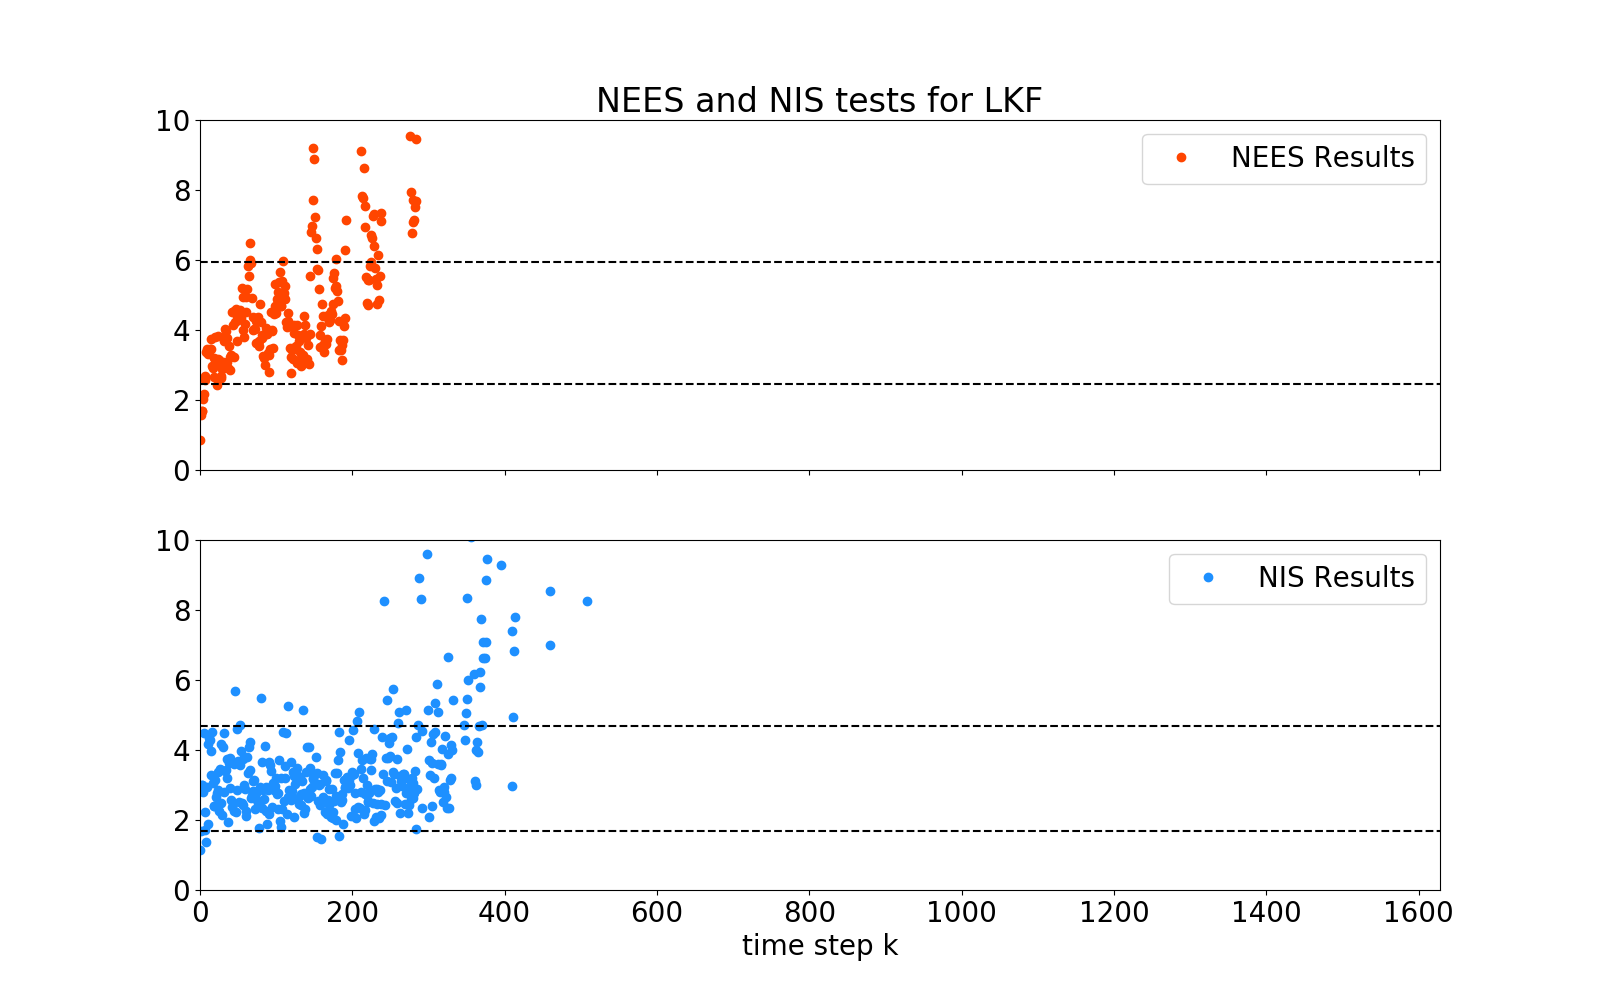
\includegraphics[width=0.8\textwidth]{./Figures/NEESNIS_lkf_N10.png}
	\caption{NEES and NIS chi-square results over time for N= \hl{N} simulated trajectories. Data points continue to grow past ~600 seconds into the analysis.}
	\label{fig:neesnis_lkf}
\end{figure}

The findings in Section I indicated that the linearized dynamics used in the LFK become invalid as small initial perturbations eventually cause large deviations from the nominal trajectory. 
Figure \ref{fig:neesnis_lkf} corroborates these findings, and solidifies our understanding of where the LKF is most capable, for small perturbations near the nominal trajectory.  


\subsection{The Extended Kalman Filter}
The EKF relies less on linearizations about an initial nominal trajectory.
Instead of linearly propagating a deviation in a state, the EKF uses full nonlinear dynamics to propagate its full current state estimate. 
It then linearizes about its current estimate, rather than the initial nominal trajectory to perform time and measurement updates to the covariance.   
This allows the EKF to adjust for small perturbations from the nominal that may grow into large devations with time, as it does not use the nominal trajectory for linearization. 
Figure \ref{fig:ekf_est} shows a time history of a typical EKF estimate. 
The EKF, in contrast with the LKF, is much more capable of tracking the perturbed trajectory.  

\begin{figure}[H]
	\centering
	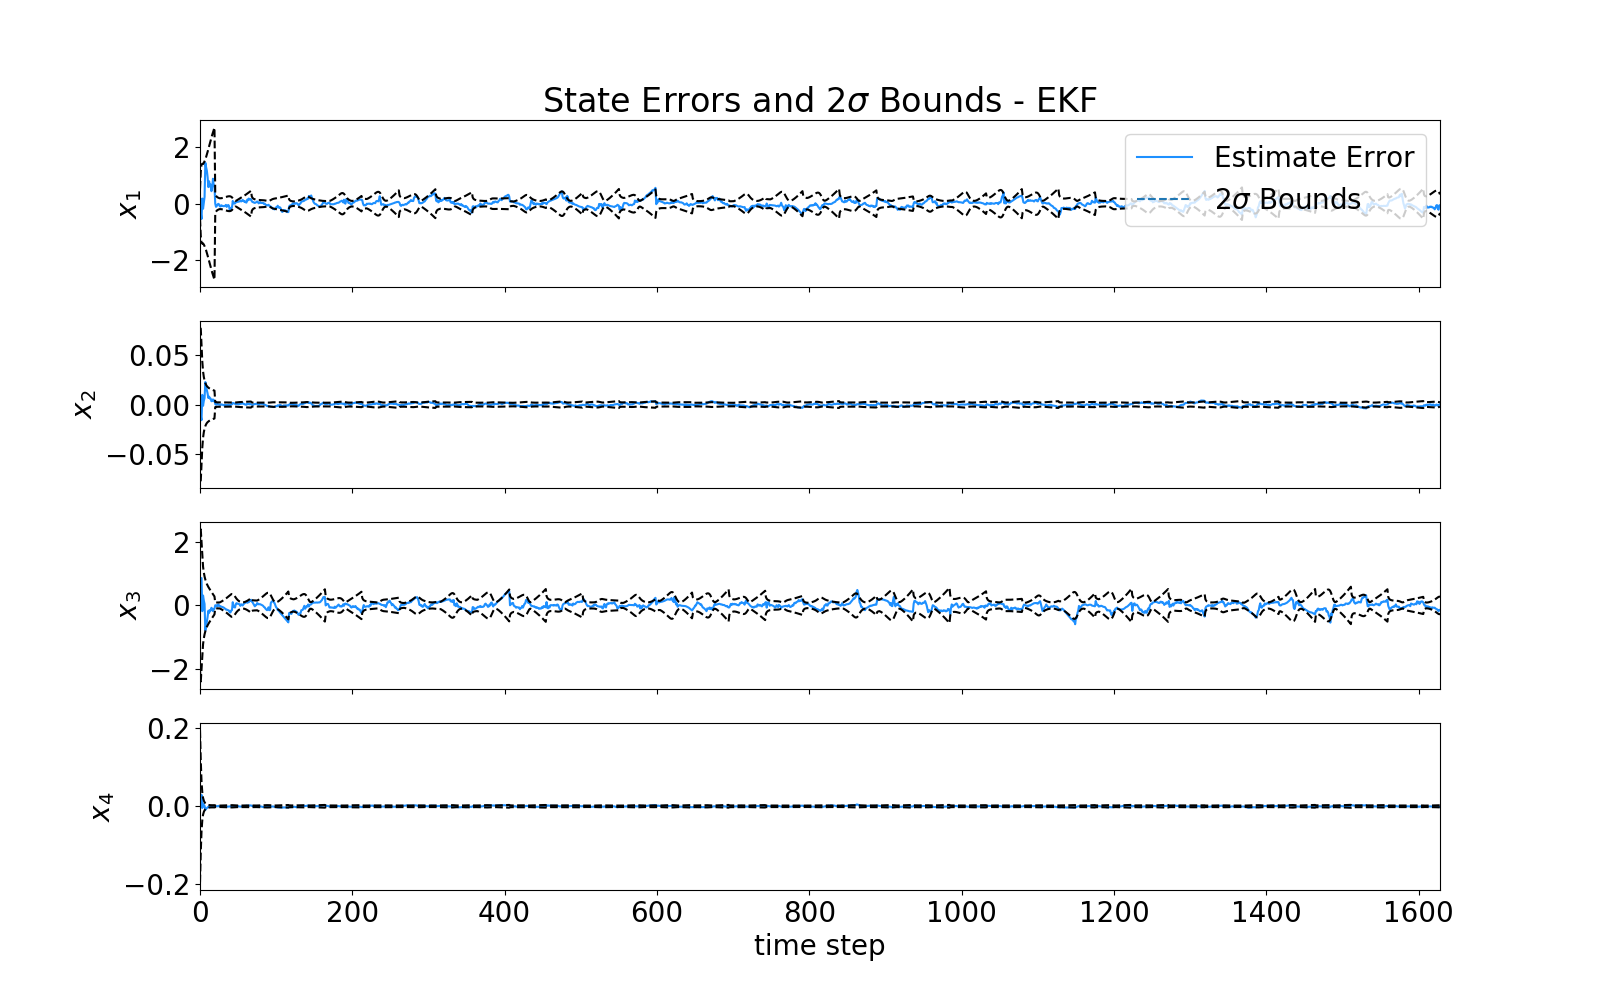
\includegraphics[width=0.8\textwidth]{Figures/ekf_estimate_th.png}
	\caption{EKF error estimate over the entire simulation period. }
	\label{fig:ekf_est}
\end{figure}


\subsubsection{NEES and NIS Tests}
Figure \ref{fig:neesnis_ekf} shows the NEES and NIS results for the EKF.
These results were generated using the same noisey trajectories and measurements as used for the LKF. 

\begin{figure}[H]
	\centering
	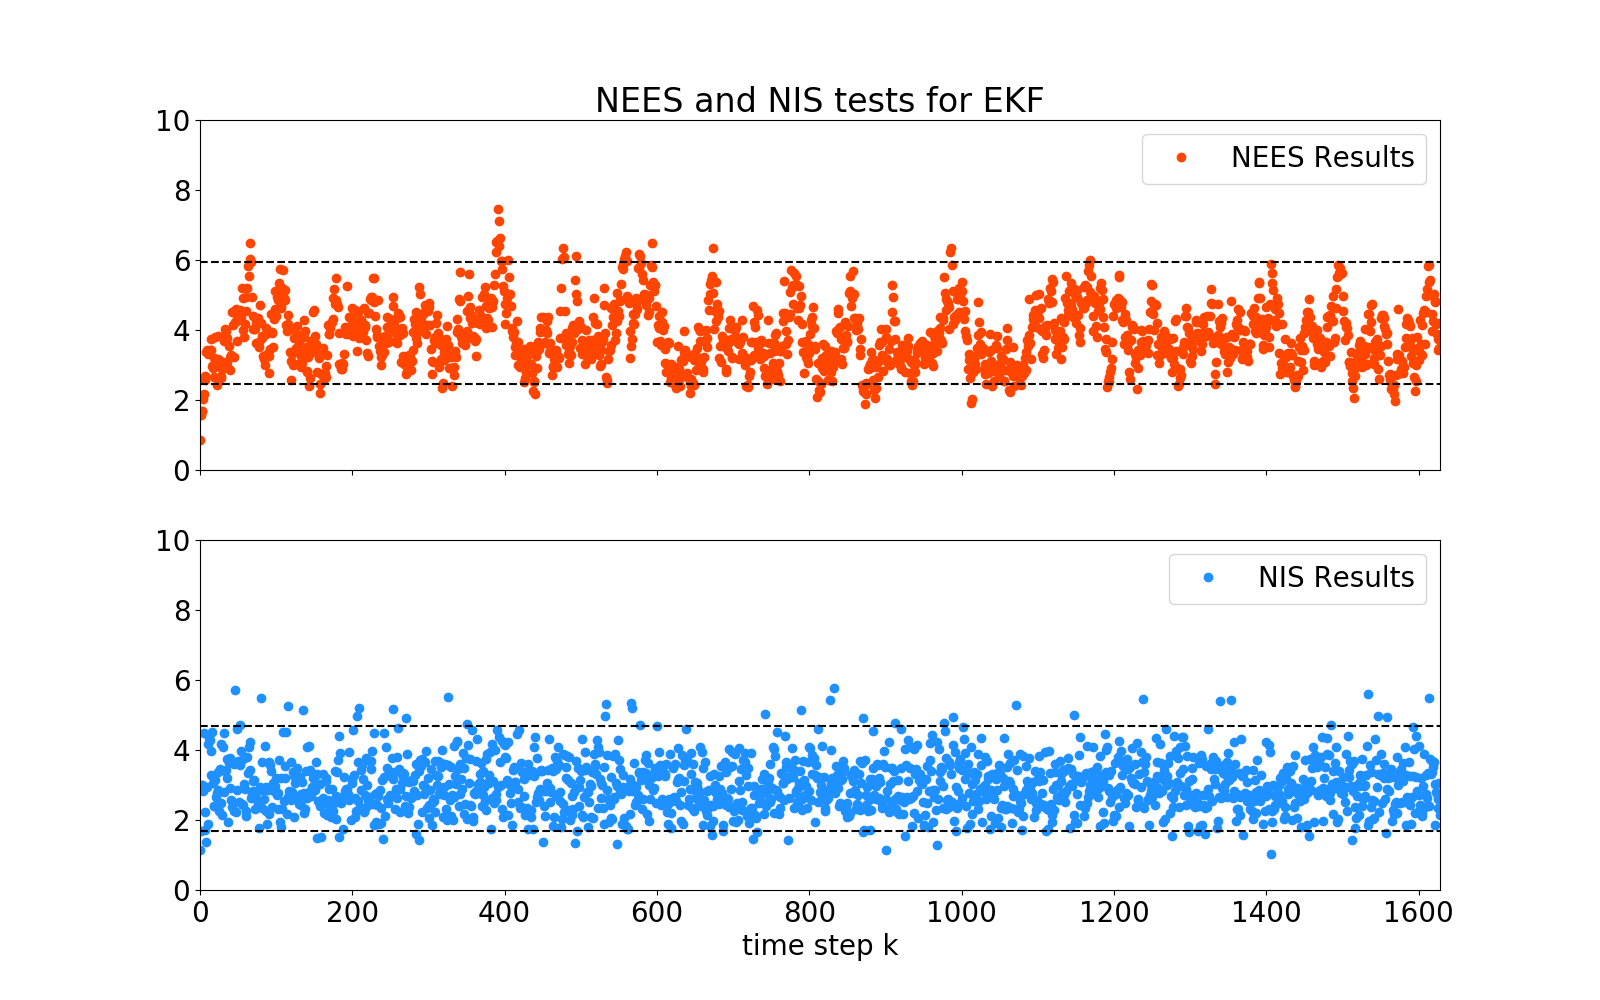
\includegraphics[width=0.8\textwidth]{./Figures/NEESNIS_ekf_N10.png}
	\caption{NEES and NIS chi-square results over time for N= \hl{N} simulated trajectories.}
	\label{fig:neesnis_ekf}
\end{figure}

These results show the estimate tracking the truth trajectory more accurately for the duration of the simulations. 
Becuase the EKF continuously updates its internal 'nominal' trajectory, it's able to latch on to the perturbed trajectory and doesn't rely on stale information from the original nominal trajectory. 
This results in the filter's ability to keep up with the deviations from the original nominal trajectory, and estimate the truth trajectory accurately.


\section{Testing Without Ground Truth}




%%%%%%%%%%%%%%%%%%%%%%%%%%%%%%%%% CONCLUSION %%%%%%%%%%%%%%%%%%%%%%%%%%%%%%%%%
\section{Conclusion}


\section{Advanced Questions}
\subsection{Bugs}
Crawling on our laptop screen \\
underneath our keyboard's keys \\
\texttt{clear all, close all, clc} \\
just end us now. Please, bugs, please. \\
 
\subsection{The Unscented Kalman Filter}


%%%%%%%%%%%%%%%%%%%%%%%%%%%%%%%%% APPENDIX %%%%%%%%%%%%%%%%%%%%%%%%%%%%%%%%%
\newpage
\section*{Appendix}
Attached here is the code used for the numerical analysis and plotting entailed in this project.
%\lstinputlisting{../main.m}


\end{document}


